\chapter{Code Snippets}
\label{chap:A2}

\subsection{Code used for Experiments in Subsection~\ref{cha:testing:onedevice}} \label{chap:A2:onedeviceclientlib}
\begin{lstlisting}[language=Rust, style=boxed, showstringspaces=false]{}
use std::error::Error;

use NOSHP_Client::{
    client::{ClientState, NoshpClient, 
        Request, UserDefinedState},
    client_config::{ClientConfig, ParsedConfig},
};

#[derive(Default)]
struct ExampleState {
    text: String,
}
impl UserDefinedState for ExampleState {}

const CONFIG_PATH: &str = "./example_config.toml";
#[tokio::main]
async fn main() -> Result<(), Box<dyn Error>> {
    let config = ClientConfig::load_config(CONFIG_PATH);
    let config = match config {
        Ok(r) => r,
        Err(e) => {
            eprintln!(
                "Error loading config: {}", e.to_string()
            );
            println!("Loading default config...");
            ParsedConfig::default()
        }
    };

    let client_handler = NoshpClient::new();
    client_handler
        .set_state(ExampleState {
            text: String::from("hello world"),
        })
        .add_callback("Turn On", Box::new(turn_on_led))
        .add_callback("Turn Off", Box::new(turn_off_led))
        .run(config)
        .await
        .unwrap();

    return Ok(());
}

fn turn_on_led(
    _state: &mut ClientState<ExampleState>,
    _req: Request
) {
    println!("Turn On")
}

fn turn_off_led(
    _state: &mut ClientState<ExampleState>,
    _req: Request
) {
    println!("Turn Off")
}
\end{lstlisting}

\pagebreak
\subsection{OS Error encountered during client spawning} 
Error when attempting to spawn 1000 clients.
\label{chap:A2:oserror}
\begin{figure}[h]
\caption{Linux TCP Error}
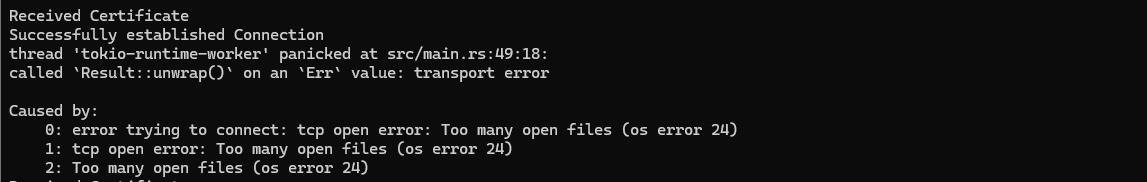
\includegraphics[width=\textwidth]{os_error_tcp_new.png}
\label{fig:tcperror}
\end{figure}


\pagebreak
\subsection{Frontend API RegistrationService Definition} \label{chap:A2:frontendApiDefinition}
\begin{lstlisting}[language=protobuf3, style=boxed, showstringspaces=false]{}
syntax = "proto3";
package frontend.registration;
import "frontendTypes.proto";

service FrontendRegistrationService {
    rpc Register(RegistrationRequest) 
        returns (RegistrationResponse);
    rpc GetConnectedDevices(ConnectedDevicesRequest)
        returns (ConnectedDevicesResponse);
};

message RegistrationRequest {
    string device_name = 1;
}

message RegistrationResponse {
    string client_id = 2;
}

message ConnectedDevicesRequest {
    string client_id = 1;
}

message ConnectedDevicesResponse {
    repeated Device devices = 1;
}

message Device {
    string device_name = 1;
    string device_uuid = 2;
    repeated frontend.types.DeviceCapabilityStatus 
        capabilities = 3;
}
\end{lstlisting}

\pagebreak
\subsection{Making API calls to the JSON Proxy} \label{chap:A2:apicallsjsonproxy}
\begin{lstlisting}[language=ES6, style=boxed, showstringspaces=false]{}
import { API_REGISTRATION_ADDRESS } from "@/api_call_links";
import { Result, errAsync, okAsync } from "neverthrow";
import { frontend } from "@/generated/generated";

export async function registerSelf(deviceName: string)
: Promise<
    Result<frontend.registration.RegistrationResponse, Error>
> {
    const req = 
        new frontend.registration.RegistrationRequest({
            device_name: deviceName,
        });

    const res = await fetch(API_REGISTRATION_ADDRESS, {
        method: "POST",
        body: JSON.stringify(req),
        headers: {
            "Content-type": 
                "application/json; charset=UTF-8",
        },
    });

    try {
        const parsed: 
            frontend.registration.RegistrationResponse =
                await JSON.parse(await res.text());
        return okAsync(parsed);
    } catch (e) {
        return errAsync(new Error("Malformed Api Response"));
    }
}
\end{lstlisting}

